\documentclass{zebracorns} 

\title{Collaborative Whitepapers Using Overleaf}
\author{The Zebracorns}
\date{September 2019}

\begin{document}

\maketitle

\section{Introduction}
Overleaf has provided The Zebracorns with a premium subscription to their software for sharing and editing \LaTeX\ (Pronounced: Lah-Teck or Lay-Teck) documents.

Before Overleaf, we were using Google Drive to write whitepapers which provided the sharing capabilities we wanted. Because Google Drive made formatting difficult, we switched to \LaTeX\ for efficient and simple formatting. We found \LaTeX\  was arduous to install locally and it restricted our collaboration. Several students began using ShareLaTeX (now Overleaf), but there was no Git integration, master templates, and the files were owned by students who graduated and left the team which meant that we lost the source code for all of our original papers.

Overleaf generously agreed to provide us with a premium subscription which allows us to keep and share the source code of our whitepapers. In this paper, we want to express our gratitude for their generosity, explain our process for writing, editing, and publishing whitepapers, and talk about the features of Overleaf that we like the most.

\section{Whitepaper Process with Overleaf}
Our process of using Overleaf includes several steps. After determining the topic and purpose of a new whitepaper\footnote{This is a complex process that involves a student or students stepping up to write something interesting to them}, we sign into Overleaf with an administrative account and create a copy of the Zebracorn Labs\footnote{\href{team900.org/labs}{team900.org/labs}} Overleaf template. The document is then shared with any team members who might be writing or editing it. After linking the Overleaf document to a GitHub repository, anyone can edit the whitepaper on Overleaf, locally, or through GitHub. We usually post the Overleaf share link in Slack\footnote{\href{slack.com}{slack.com}}, our team communication system. Multiple team members then work together to outline the paper and draft the sections. Thanks to the unique features of Overleaf and the collaborative nature of source control, different people can work on different sections at once.

In drafting the paper, we make extensive use of the fact that Overleaf is a \LaTeX\ editor. We organize content by sections and subsections, helping break down the paper for readers. Our template automatically generates a table of contents; this is useful when we change sections around, which happens frequently throughout our creative process. We use footnotes, text formatting (code, monospace, italics, bold, etc.), figure insertion, and the glossary function to write our papers.

Both during drafting and afterwards, we edit and revise our paper. We use the ability to leave comments on text to communicate feedback. The person who wrote the section in question can come back and revise, or reply to the comments to discuss the issue. Others can see the comment and add their input.

\begin{figure}[h]
  		\centering
  		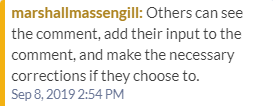
\includegraphics{Comment.PNG}
\end{figure}

We only publish the paper when everyone editing, reviewing, revising, and commenting on the paper is satisfied. We download a PDF from Overleaf, add it to our Google Team Drive, and post the link to the PDF on our website\footnote{Our website is hosted on Github pages so it's a simple process to edit the links and publish new content.}. You can find all of the whitepapers that we've posted \href{team900.org/labs}{here}. We also post the PDF link on Chief Delphi, the (Un)Official FIRST Robotics Competition forum, where other members of the community can read and comment on the papers.

\section{Features}
In the time we've been using Overleaf for documentation, we've grown to appreciate many of the features of the software and the collaboration that it enables for us. 

Since our robotics team regularly publishes at least one or two papers a year, we place a lot of emphasis on the continuity of our documentation. It makes it a lot easier to understand previous years' work when the formatting is consistent throughout years. Using \LaTeX\ with Overleaf has allowed us to reference a \LaTeX\ template to exactly replicate the formatting. It also allows our papers to have a uniform, clean, professional appearance without the writers having to spend a lot of time in formatting. 


We also appreciate Overleaf's ability to enable multiple editors at once and to have editors make comments in the Overleaf document. We try to include everyone we can in the writing and editing of our yearly whitepapers, because summarizing the work of the year helps with understanding that work better. It also serves to bring new team members into the process and introduce them to new technologies. The ability to have seven different students and mentors reading, writing, and editing the paper in real time during robotics meetings  matches remarkably well with the collaborative nature of The Zebracorns. 

When we first started using Overleaf, we would mainly share PDFs of the documents for revision in Slack. We quickly realized that it was difficult to keep track of changes we had made and to access previous versions. With Overleaf Premium, we're able to use the history feature to see previous versions of the document. The ability to view the revision history makes it possible to have many different editors without cluttering our Slack channels with ``WhitepaperFinal.pdf'', ``WhitepaperFinalFinal.pdf'', and ``WhitepaperFinalFinalv2.pdf'', and
``WhitepaperFinalFinalNoReallyThisTime-v9.pdf'' eternally. (Those are real examples of file names we have used.)

We also make use of Overleaf Premium's GitHub integration. We publish our whitepaper source code to GitHub while we're working on the paper and when we've completed it. This allows team members to edit the source code locally, if they want to. It also allows us to open-source the code for our whitepapers if we choose.

\section{Features We Want}
As we have used Overleaf, we have thought of some features we would like to see added. One of these features is not requiring an account to view or comment on an overleaf document. This makes it easier for people who want to skim the document for formatting or grammar, but do not regularly write or edit documents on Overleaf.

Another feature we would like is for Overleaf to mass-update document templates. Currently, when we make a change to a template, it will only exist for all future papers created from the template. If we wanted to make the change retroactively, to say, change our primary font, we would have to edit each paper individually. 


\section{Outcomes}
We've published a few papers using Overleaf, the most recent being our 2019 programming paper, an update on our activities with ROS (Robot Operating System). That whitepaper can be found \href{https://team900.org/blog/ZebROS1.1/}{here}. Overall, our papers have been downloaded thousands of times by members of our robotics community and beyond. They serve as references for people outside of the robotics team, and as internal documentation of our progress each year. They even help us maintain our partnerships with our sponsors by showcasing our work and their products or services.

We would like to thank Overleaf for providing us with this software, which has allowed us to write and edit professional, consistent whitepapers for documentation and to share our knowledge. Our whitepaper process wouldn't be the same without Overleaf!

\end{document}
